\documentclass[tikz,border=5pt]{standalone}
\usepackage{tikz}
\usetikzlibrary{shapes.geometric, arrows.meta, positioning, fit, backgrounds, calc}

\begin{document}
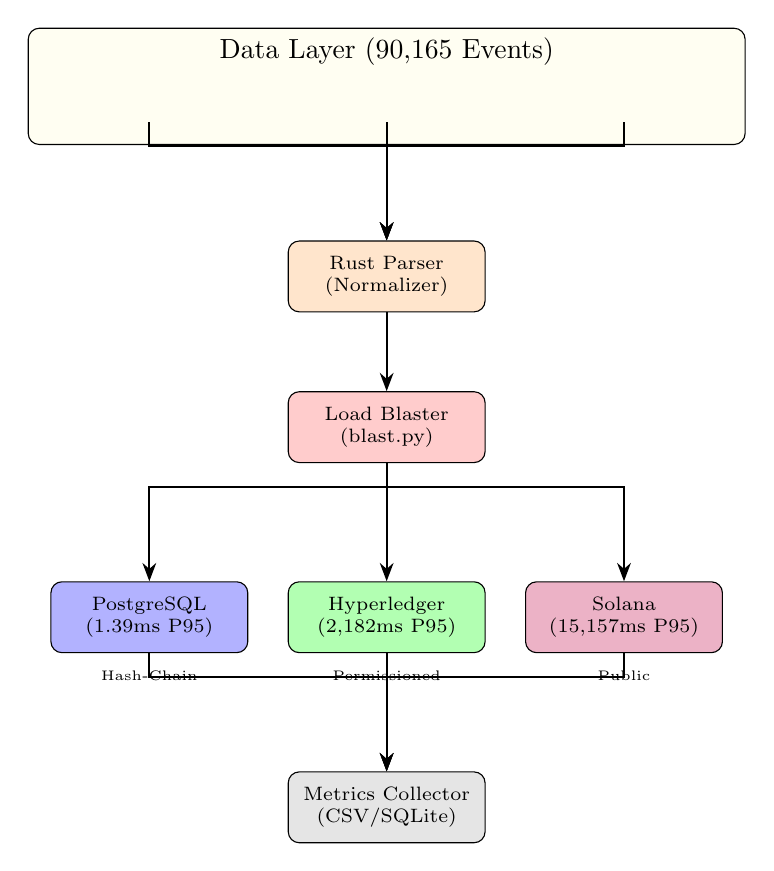
\begin{tikzpicture}[
    node distance=1cm and 1.5cm,
    box/.style={
        rectangle,
        draw,
        rounded corners,
        minimum width=2.5cm,
        minimum height=0.9cm,
        align=center,
        font=\scriptsize
    },
    layer/.style={
        rectangle,
        draw,
        rounded corners,
        inner sep=8pt,
        font=\small\bfseries
    },
    arrow/.style={
        ->,
        >=Stealth,
        thick
    },
    doublearrow/.style={
        <->,
        >=Stealth,
        thick
    }
]

% Data Layer
\node[box, fill=yellow!20] (dataset1) {UAV Attack\\Dataset};
\node[box, fill=yellow!20, right=0.5cm of dataset1] (dataset2) {Cyber-Physical\\IoD Dataset};
\node[box, fill=yellow!20, right=0.5cm of dataset2] (dataset3) {CICIoV2024};

\node[layer, fill=yellow!5, fit=(dataset1)(dataset2)(dataset3), label={[anchor=north]north:Data Layer (90,165 Events)}] (datalayer) {};

% Parser
\node[box, fill=orange!20, below=1.5cm of dataset2] (parser) {Rust Parser\\(Normalizer)};

% Event Generator
\node[box, fill=red!20, below=1cm of parser] (generator) {Load Blaster\\(blast.py)};

% Target Systems
\node[box, fill=blue!30, below left=1.5cm and 0.5cm of generator] (postgres) {PostgreSQL\\(1.39ms P95)};
\node[box, fill=green!30, below=1.5cm of generator] (hyperledger) {Hyperledger\\(2,182ms P95)};
\node[box, fill=purple!30, below right=1.5cm and 0.5cm of generator] (solana) {Solana\\(15,157ms P95)};

% Metrics
\node[box, fill=gray!20, below=1.5cm of hyperledger] (metrics) {Metrics Collector\\(CSV/SQLite)};

% Arrows from data to parser
\draw[arrow] (dataset1.south) -- ++(0,-0.3) -| (parser.north);
\draw[arrow] (dataset2.south) -- (parser.north);
\draw[arrow] (dataset3.south) -- ++(0,-0.3) -| (parser.north);

% Parser to generator
\draw[arrow] (parser) -- (generator);

% Generator to systems
\draw[arrow] (generator.south) -- ++(0,-0.3) -| (postgres.north);
\draw[arrow] (generator) -- (hyperledger);
\draw[arrow] (generator.south) -- ++(0,-0.3) -| (solana.north);

% Systems to metrics
\draw[arrow] (postgres.south) -- ++(0,-0.3) -| (metrics.north);
\draw[arrow] (hyperledger) -- (metrics);
\draw[arrow] (solana.south) -- ++(0,-0.3) -| (metrics.north);

% Labels for systems
\node[below=0.1cm of postgres, font=\tiny] {Hash-Chain};
\node[below=0.1cm of hyperledger, font=\tiny] {Permissioned};
\node[below=0.1cm of solana, font=\tiny] {Public};

\end{tikzpicture}
\end{document}
